\documentclass[journal]{IEEEtran}

% *** CITATION PACKAGES ***
%
%\usepackage{cite}
\usepackage{capt-of}%%To get the caption
\usepackage{gensymb}
\usepackage{graphicx} %package to manage images
\graphicspath{ {./images/} }
\usepackage{wrapfig}

\usepackage{amsmath}
\usepackage{amssymb}

\usepackage{lipsum}

\usepackage[style=ieee]{biblatex}
\DeclareLanguageMapping{english}{english-apa}
\addbibresource{references.bib}
\usepackage[justification=centering]{caption}

\usepackage{setspace}

\usepackage{hhline}


\usepackage{changepage} 

\usepackage{booktabs}
\usepackage{xcolor}

\usepackage{makecell}
\usepackage{graphicx,subcaption}
\usepackage{listings}
\renewcommand\theadfont{}
\DeclareMathOperator{\EX}{\mathbb{E}}% expected value


\usepackage{multicol} 

\raggedbottom

\begin{document}


\pagenumbering{gobble}
%\clearpage\mbox{} % adds and empty page
%\clearpage
\pagenumbering{arabic}
\setcounter{page}{1}

\title{Simulating Network Architectures}

\author{ ENGR-UH 2010Q Probability and Statistics, Fall 2019\\
\medskip
Barkin Simsek,~\IEEEmembership{bs3528@nyu.edu};
Nishant Aswani,~\IEEEmembership{nsa325@nyu.edu}}% <-this % stops a space


% The paper headers
\markboth{Simsek, Aswani, ENGR-UH 2010Q Probability and Statistics, Fall 2019}%
{}

% make the title area
\maketitle

% As a general rule, do not put math, special symbols or citations
% in the abstract or keywords.
\begin{abstract}
With the rapid development of computer networks, various ways of connecting computers to each other have been established and created computer networks. These networks can have different architectures depending on miscellaneous constraints such as budget, bandwidth, speed, etc. In this project, network architectures that follow power laws (scale-free networks) and Poisson distribution (random networks) are simulated and analyzed in terms of connectedness (speed) and service time (message drop).

\end{abstract}

%%%%%%%%%%%%%%%%%%
%% Introduction %%
%%%%%%%%%%%%%%%%%%
\section{Introduction}
\subsection{Problem Description}
\IEEEPARstart{N}\lowercase{etworks} are an integral part of describing natural and artificial systems, such as networks of neurons in our brain or computer networks. In today's heavily interlinked world, everything with a capability of connection has somehow already been connected. While this may seem like a trivial statement, its implications are far more profound. How elements of a network are connected plays a crucial importance in the network's efficiency, health, and resilience against failures. For example, in the 2003 North American Blackout, a local failure in Ohio caused the entire North American power grid network to go down, leaving millions of people in the dark \cite[]{blackout}. Experts say that this could have prevented if the power grid network was developed with a better structure in mind. Similarly, computer networks are prone to such cascading failures as well but are often prevented due to their distributed structure and built-in redundancies. The spread of a cascading failure in a network is depicted in Figure \ref{fig:failure}. \\

\begingroup
    \centering
    \medskip
    %width=\columnwidth
    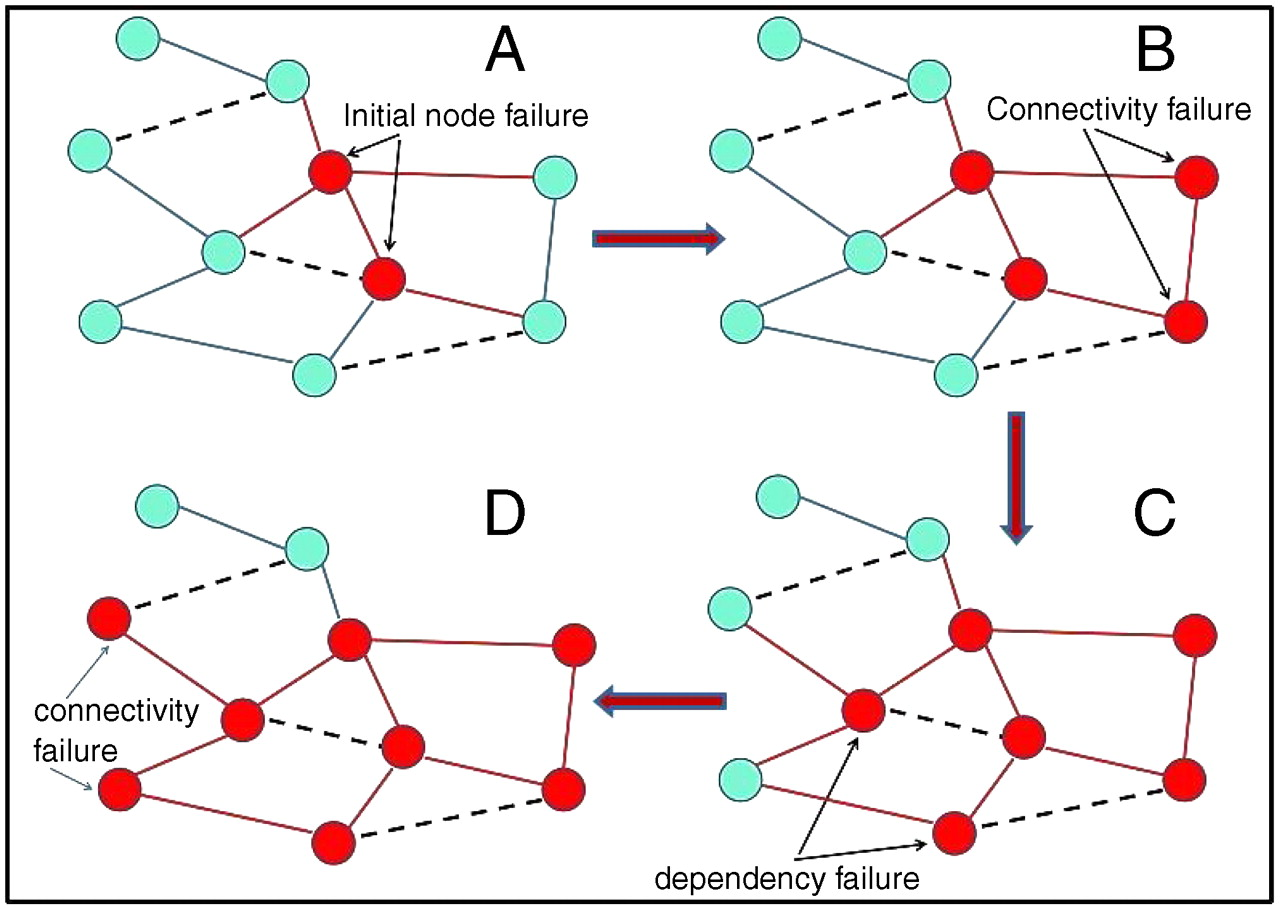
\includegraphics[width=\columnwidth]{images/failure.jpg}
    \captionof{figure}{Cascading failures in networks \cite[]{Parshani_Buldyrev_Havlin_2011}}
    \label{fig:failure}
    \medskip
\endgroup

\noindent As a result, analysis and modeling of various network structures before building a system becomes imperative. Often times, several constraints must be kept in mind. For example, building a network where each node is connected to every other node might help us tolerate local failures in the network; however, the cost of such a network may not be feasible. Furthermore, there might be other constraints like privacy between nodes of the network or number of connections that can be made between nodes in a network.\\

\noindent This project was inspired by a larger inquisition in how to connect a network of autonomous vertical farming units. We began by questioning whether the needs of our system would be best met by a decentralized network or a distributed network. Figure \ref{fig:network_types} depicts the three major types of networks. \\

\begingroup
    \centering
    \medskip
    %width=\columnwidth
    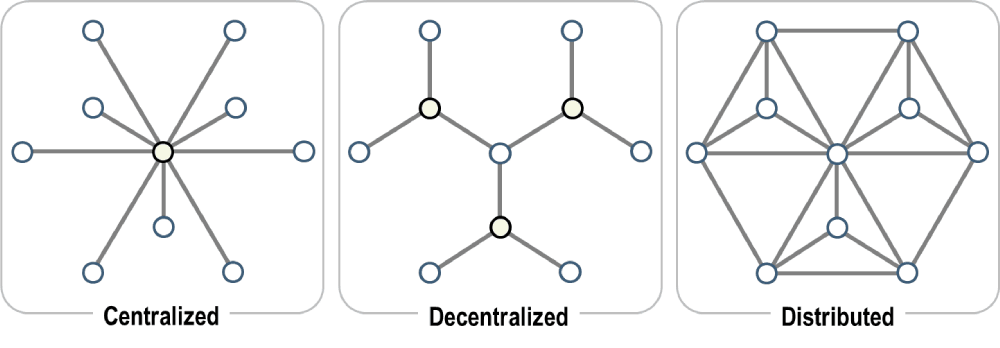
\includegraphics[width=\columnwidth]{images/network-structures.png}
    \captionof{figure}{Three main groups of networks \cite[]{U_L_2001}}
    \label{fig:network_types}
    \medskip
\endgroup

\noindent A decentralized network operates on the idea of sub-centers, where each of the sub-centers acts as a mini-hub for several other minimally connected nodes. These sub-centers are fully connected amongst themselves. \\

\noindent On the other hand, a distributed system implies a high-level of inter-connectivity, lacking the concept of centers of communication. This also brings along redundancy \emdash node A could communicate with node Z through multiple paths with varying distances \cite{Network_Structure_2017}. \\

\noindent When brought into the realm of network science, we determined that the scale-free system best represents a decentralized network, as it results in a set of highly connected nodes. We also decided to use a random network to simulate the distributed network. 




%%%%%%%%%%%%%%%%%%%%%%%%%%%%%%%%%%%%%%%%%%%%%%%%%%%%%%%%%%%%%%%%%%
% \textbf{Text below is just copy - paste, we need to change is a little bit}
% Centralized. One center has high accessibility and thus represents the dominant element of the network and the spatial structure it supports. This is the common characteristic of hub and spoke networks.

% Decentralized. Although the center is still the point of highest accessibility, the network is structured so that sub-centers have also significant levels of accessibility.

% Distributed. No center has a level of accessibility significantly different from the others, which implies a high connectivity levels and redundancy.
%%%%%%%%%%%%%%%%%%%%%%%%%%%%%%%%%%%%%%%%%%%%%%%%%%%%%%%%%%%%%%%%%%


\begin{figure*}[!ht]
\end{figure*}

%%%%%%%%%%%%%%%%%%%%%%%%%%%%%%%%%%%%%%%%%%%%%%%%%
%% Probability Distribution of Chosen Networks %%
%%%%%%%%%%%%%%%%%%%%%%%%%%%%%%%%%%%%%%%%%%%%%%%%%
\section{Probability Distribution and Network Architecture}
% \subsection{Network Architecture that Follows a Poisson Degree Distribution}
\subsection{Random Networks}

\noindent Random networks are generated with links between nodes being assigned randomly. One of the models for random network generation, used by Erdős and Rényi, fixes the number of nodes and edges within the network \cite{barabasi2016network}. \\

\noindent Network generation then involves iterating through a list of available edges and randomly selecting two nodes to link at each iteration. In a given iteration, if two selected nodes are already connected, then two random nodes are selected again (see Appendix A). As a result of this method, the network generated is truly random, even including cases where specific nodes miss out on any connections. Moreover, empirically, a random network (see Figure \ref{fig:random_histogram}) results in a well-spread degree distribution, lacking cases of nodes holding an extreme degree. Looking at the histogram representation (see Figure \ref{fig:random_network}) of the degree distribution, we see that it may be modeled by a Poisson or Binomial distribution.\\

\noindent To describe the degree distribution of a random network, we first establish that a Poisson distribution is a special case of the Binomial distribution, where $n \rightarrow \infty$ and the chance of success in each trial approaches 0. In the Poisson distribution equation below, n refers to the number of nodes, while $\lambda$ refers to the mean degree.\\

\begin{equation}
    \begin{split}
        P(\lambda, n) = (\frac{\lambda^n e^{-\lambda}}{n!})
    \end{split}
    \label{eq:poisson_distribution}
\end{equation}
\\

\noindent Since we are using a Poisson distribution, it is given that the number of nodes is large. Calculating the $\EX(k)$, we see that it results in $\lambda$. 

\begin{equation}
    \begin{split}
        X &\texttt{\char`\~} Poisson(\lambda) \\
        \\
        P(X=k) &= \frac{\lambda^k e^{-\lambda}}{k!} \\
        \\
        \EX(k) &= e^{-\lambda}\sum_{k=1}^{\infty} \frac{\lambda^n}{(n-1)!}\\
        \\
        &= e^{-\lambda}\lambda\sum_{k=1}^{\infty} \frac{\lambda^{k-1}}{(k-1)!}\\
        \\
        &= e^{-\lambda}\lambda\sum_{n=0}^{\infty} \frac{\lambda^{n}}{(n)!}\\
        \\
        &= e^{-\lambda}\lambda e^{\lambda} = \lambda\\
    \end{split}
    \label{eq:mutual}
\end{equation}

\noindent Hence, we know that the $\lambda$ parameter can be approximated as the mean degree.

\begin{equation}
    \begin{split}
        \lambda = \frac{\sum_{i=1}^{n}D_i}{n}
    \end{split}
    \label{eq:poisson_distribution}
\end{equation}


% \subsection{Network Architecture that Follows a Power Law Distribution}
\subsection{Scale-Free Networks}
\noindent However, random networks ignore the paradigm where node popularity is a factor. The internet serves as a common example, where certain devices act as hubs for other devices to connect to the larger network. Hence, we introduce the scale-free model, which has several variations, but operates on the principle of preferential attachment. Preferential attachment can colloquially be described as "the rich get richer." Essentially, new nodes are more likely to connect to older nodes, making the older nodes more popular. As this project attempts to meet an edge budget, we use a slight variation of the Barabási–Albert model.\\

\noindent Ten fully inter-connected nodes are selected to form the initial network. Iterating through the remaining nodes, a node is selected to add to this network. The new node makes $\frac{\text{totalEdges}}{\text{remainingNodes}}$ connections to attempt meeting the budget, picking the most popular nodes to connect with. Popularity in our network is determined by $\frac{\text{nodeDegree}}{\text{2*numberOfEdges}}$, which gives a probability value. We then select a node to connect with based on the probability values of all nodes within the network. Once a node has been added, it is considered for connection in the next iteration (see Appendix B). As a result, we obtain a network with visibly popular nodes (see Figure \ref{fig:scalefree_network}). \\

\noindent The degree distribution of a scale-free network follows the power-law distribution. When $ 2 < \gamma < 3$, we obtain a network with a well-defined mean and infinite variance. This implies that there is a long tail, or there exist nodes with a relatively huge degree.

\begin{equation}
    \begin{split}
        P(n) \propto ak^{-\gamma}
    \end{split}
    \label{eq:poisson_distribution}
\end{equation}


\noindent However, in the case where $\gamma > 3$, the variance is finite. This means that the model actually converges to a Normal distribution. 


%%%%%%%%%%%%%%%%%%
%% Metrics Used %%
%%%%%%%%%%%%%%%%%%
\section{Metrics Used}
\noindent Since computer networks are the main focus of this project, \textit{service time} and \textit{connectedness} were decided to be the metrics that would be used to compare these two network types. Both of these metrics are important to benchmark before deciding on which type of network is more suitable for a given application and a budget. These two metrics are especially important among the other ones since they affect the network quality perceived by the end-user directly \cite{Yamamoto_Beerends}.

\subsection{Service Time}
\noindent Every node on a computer network has a limited bandwidth and storage for transferring the message to another node. Every node on the network can transfer incoming messages without experiencing any message drop as long as the bandwidth/storage limit of the corresponding node is not reached. If the capacity is reached, the node will not be able to process the incoming messages, and message drop will occur. As a result, there will be a delay in the service since dropped messages need to be recovered, and it is a process that takes time. Any extra time required to process messages in the network affects the overall service time. Therefore, the service time is substituted as a measurement for the message drop metric for this project.\\

\noindent In the experiments, service time is directly related to the inverse of the node degrees since all edges between the nodes have the same weights, and all nodes considered to be equal in terms of capacity. Thus, a node with a higher number of connections is more likely to experience more message drop and higher service time since the capacity would be filled faster. On the other hand, nodes with fewer connections are more likely to stay under the node capacity and successfully deliver all messages. As shown in Figure \ref{fig:message_drop_explained}, all nodes in the network have the same message capacity, and all edges between the nodes can carry the same amount of message. That being said, the node in the middle (the red one) is more likely to have a message drop since all six messages can come at the same time. On the other hand, the node at the right top corner (the green one) wouldn't have message drop at all since it might receive two messages maximum and it has the capacity of four messages.\\

\begingroup
    \centering
    \bigskip
    %width=\columnwidth
    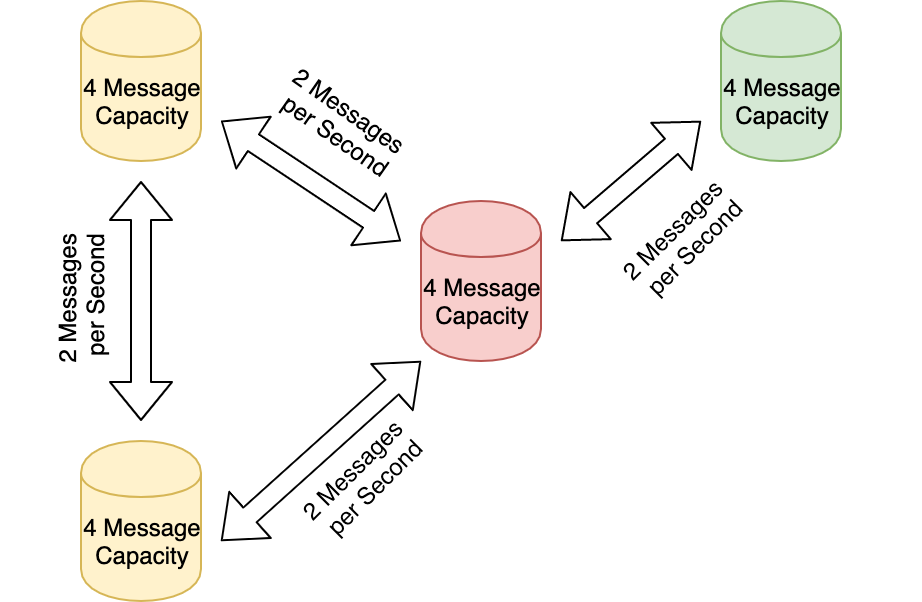
\includegraphics[width=\columnwidth]{images/message_drop.png}
    \captionof{figure}{Message drop in the network explained. Cylinders represent the nodes and the arrows represent the edges between the nodes.}
    \label{fig:message_drop_explained}
    \bigskip
\endgroup

\noindent Therefore, the service time is defined as the inverse of the node degrees as shown below:

\begin{equation}
    e^{-D_n}
    \label{eq:service_time_eq}
\end{equation}

\subsection{Connectedness}
\noindent Connectedness is another very important measure in a network since it affects the speed of a message moving in the network. Messages can move faster in a network that has many connections between every node. If a message needs to pass through many nodes or travel very long distances while going from node A to B, the network will be slower. Even though we can connect every single node with each other, creating connections between has a cost as well. This cost might be in terms of memory usage, cable usage, etc. Therefore, we need to use connectedness as a measure for speed and find the middle ground between connecting all nodes and staying within the budget. \\

\noindent In the experiments, it is assumed that every link between nodes has the same length. Therefore, the average distance between every node in the network will give us an idea about how connected the network is. Since we assume the length of each connection the same, we can also use the connectedness as a measure for the average speed of a message moving in the network. For example, Figure \ref{fig:connectedness_explained} shows two different types of networks. The one on the left has a connection between every single node, while the one on the right has connections through the center hub node. If we want to send a message from node A to B, we only need to go through one edge (the blue arrow). On the other hand, going between nodes A and B requires us to pass through two edges and a node (shown in blue). So, a message can move faster on the network shown on the left because it needs to go through a single link in a given unit of time.\\

\begingroup
    \centering
    \bigskip
    %width=\columnwidth
    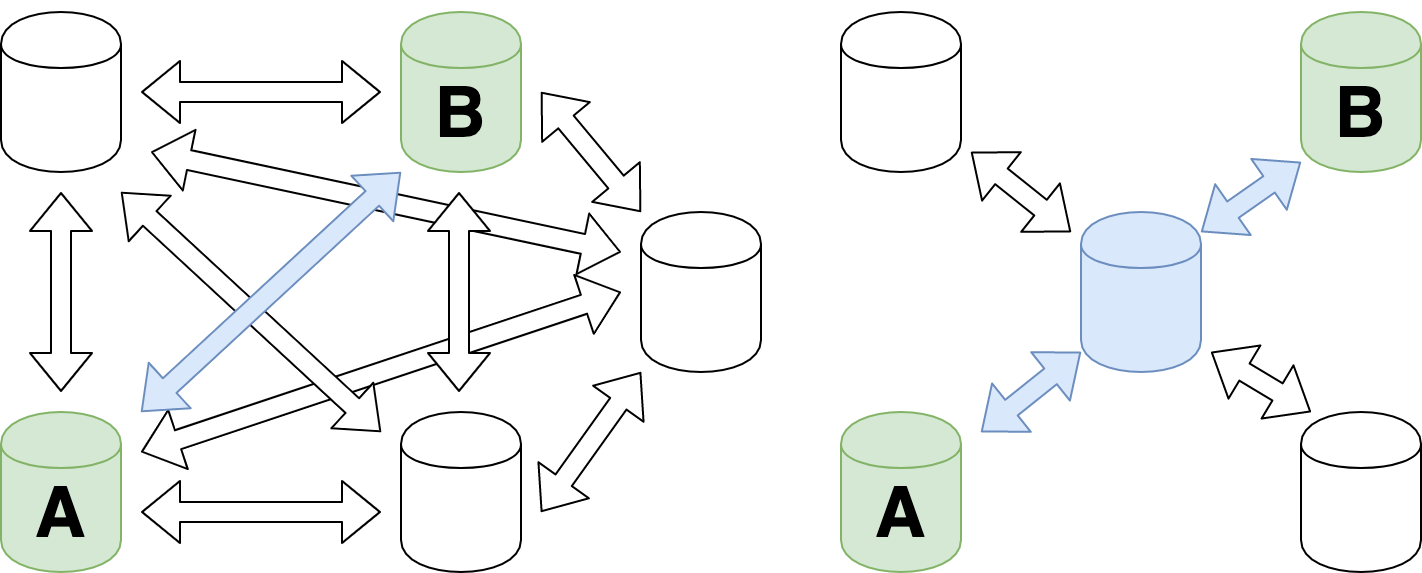
\includegraphics[width=\columnwidth]{images/speed.png}
    \captionof{figure}{Connectedness of the network explained. Cylinders represent the nodes and the arrows represent the edges between the nodes.}
    \label{fig:connectedness_explained}
    \bigskip
\endgroup

\noindent Therefore, the connectedness of the network is directly proportional to the speed of a message moving in the network and it is represented with the average distance between any nodes in the experiments as shown below:

\begin{equation}
    e^{-D_n}
    \label{eq:connectedness_eq}
\end{equation}

%%%%%%%%%%%%%%%%%%%%%%%%%
%% Experimental Method %%
%%%%%%%%%%%%%%%%%%%%%%%%%
\section{Experimental Method}
\noindent The network architectures explained above were tested with the NetworkX library in Python. Shown in Appendix A and described in Section 2, the algorithm for random network was built and tested to requirements. Next, the first version of a scale-free network was built (see Appendix C). In this iteration, $N$ nodes were initialized and were assigned equal probabilities. In the first iteration, two random nodes were chosen and were rewarded by increasing their probability values. In later iterations, the algorithm was choosing two random nodes considering the probability values attached to them, and these nodes were getting connected and getting rewarded. Unfortunately, this did not lead to a scale-free network. We then switched to the method described in Section 2.\\

\noindent After completing coding the algorithms that create networks we wanted, we started by running 100 simulations per each network type. We decided to create 50,000 nodes and 100,000 in each simulation. After running the simulation for 2 hours not even completing one iteration of the simulation, we realized that it would not be possible for us to complete all simulations before the project deadline. By experimentally reducing the node and edge sizes, we decided to run 50 simulations per each network and use 5,000 nodes and 10,000 edges. \\

\noindent We run the 50 simulations per each network type and it took more than 20 hours of computing to finish the simulations. Later, we used seaborn library in Python to graph the data we have collected. We also used Gephi software to visualize the networks we have simulated. We have used the NetworkX's builtin \texttt{shortest\_path\_length} function two measure the distance between the nodes and calculate the average value for determining the connectedness. Finally, we used NetworkX's builtin \texttt{degree} function to get the degree associated with every node in the network and determine the service time metric for the networks.

\newpage
%%%%%%%%%%%%%
%% Results %%
%%%%%%%%%%%%%
\section{Results}

\subsection{Random Network}

\noindent Figure \ref{fig:random_histogram} depicts the results of five runs with 500 nodes and 1500 edges, while Figure \ref{fig:random_network} shows a node visualization of a single run.   

\begingroup
    \centering
    \medskip
    %width=\columnwidth
    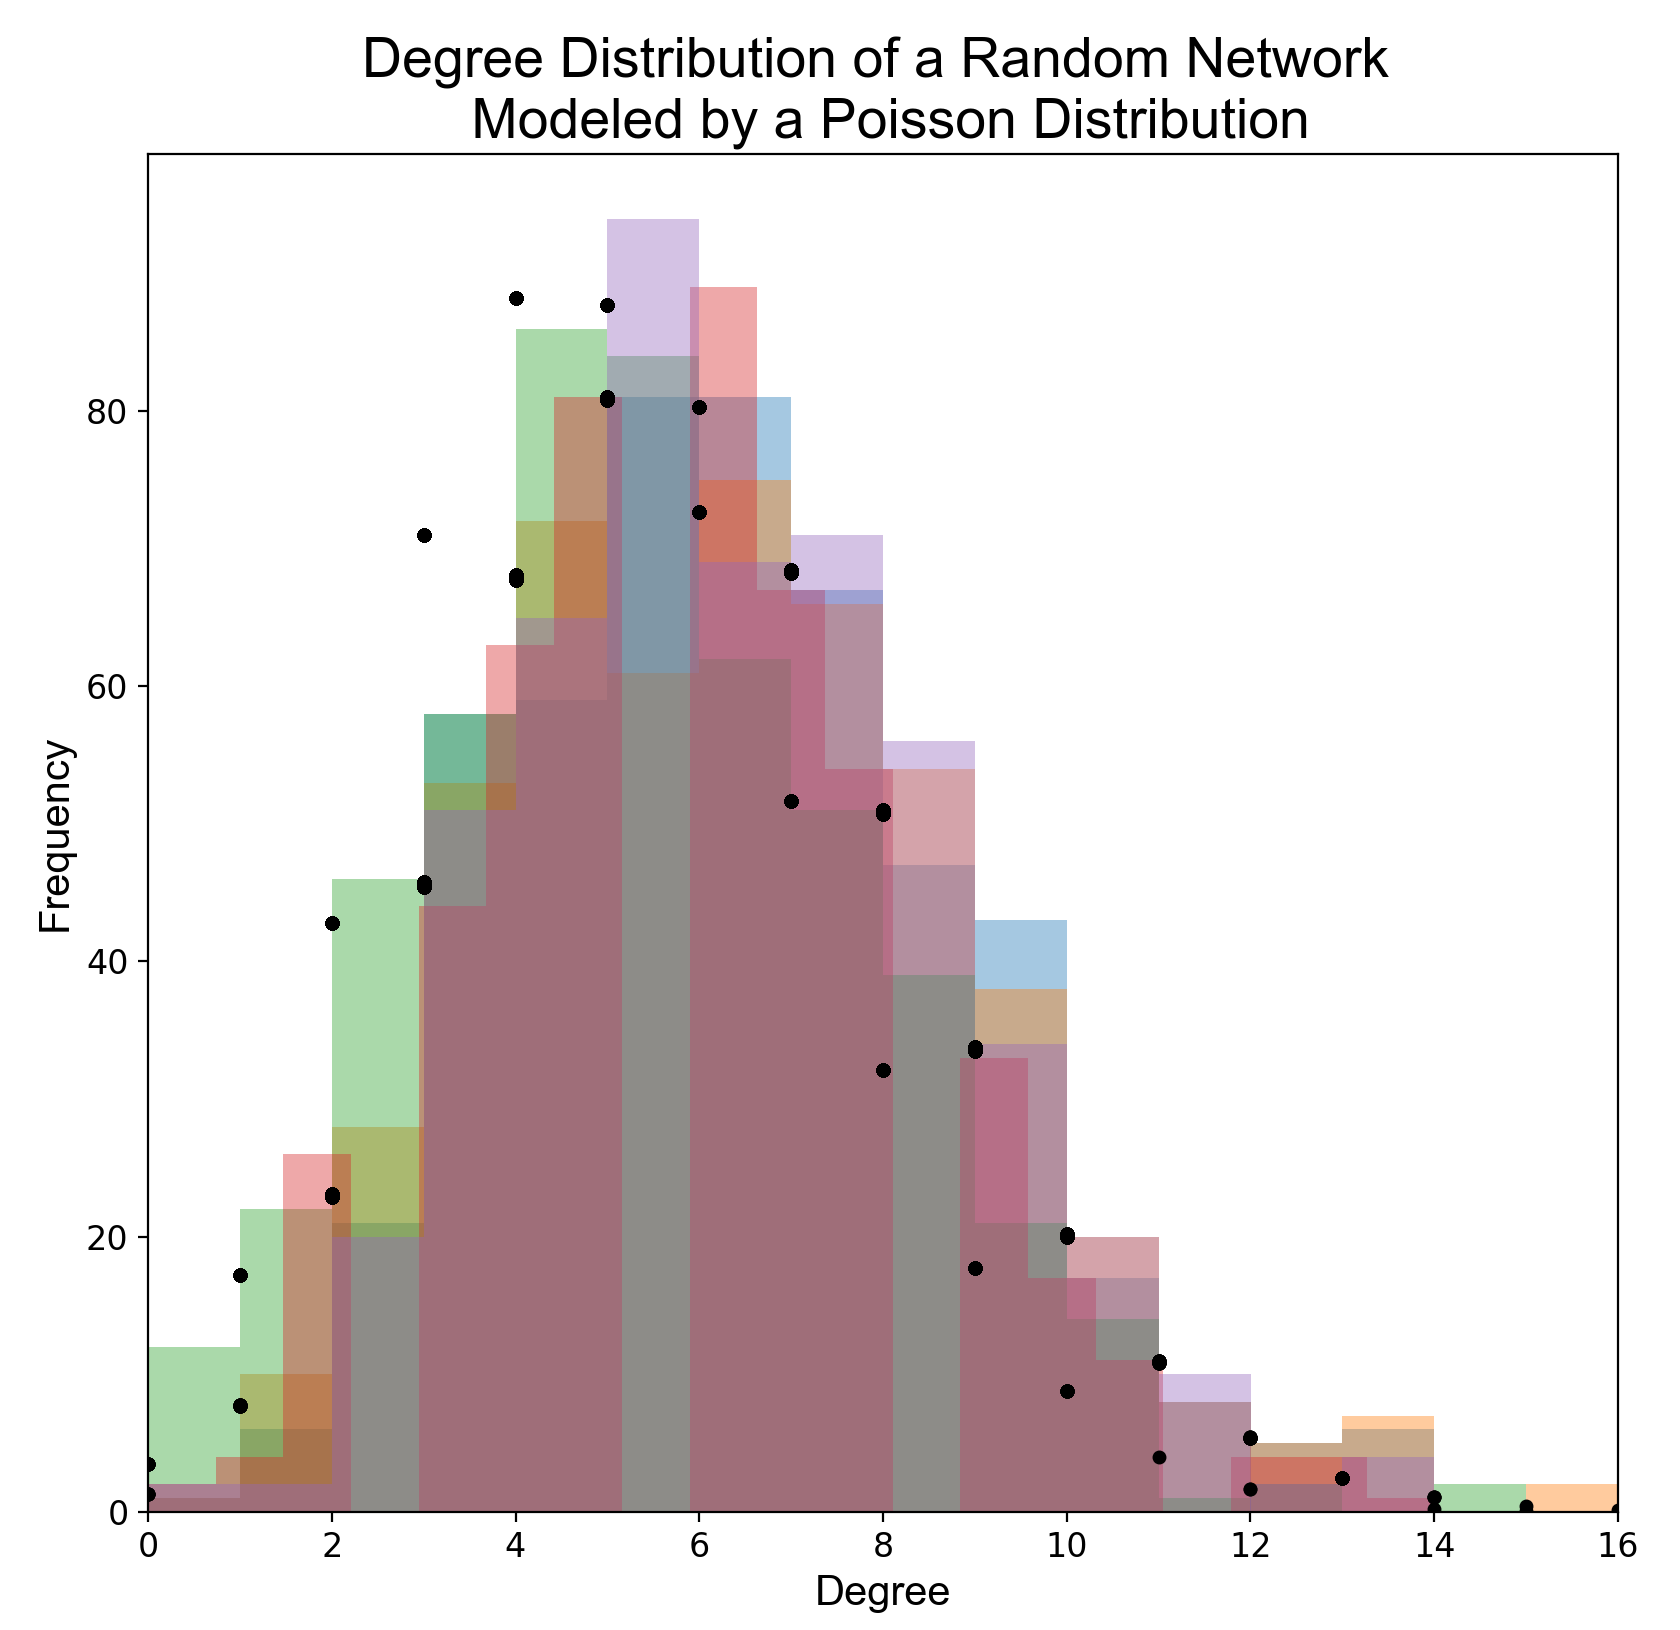
\includegraphics[width=\columnwidth]{images/rand_dist_5.png}
    \captionof{figure}{Five overlayed histograms of random networks with n=500, e=1500}
    \label{fig:random_histogram}
    \medskip
\endgroup

\bigskip
\bigskip
\bigskip

\begingroup
    \centering
    \medskip
    %width=\columnwidth
    \includegraphics[width=\columnwidth]{images/random.png}
    \captionof{figure}{Random network with n=500, e=1500. Size and color of each is proportional to that node's degree. Bigger and darker node have more connections. Smaller and lighter nodes have fewer connections.\\}
    \label{fig:random_network}
    \medskip
\endgroup

\newpage

\noindent Figure \ref{fig:fifty_average_random_degree} shows the average degree in a random network for 50 runs \ref{fig:fifty_average_random_distance} shows the average distance in a random network for 50 runs.


\begingroup
    \centering
    \medskip
    %width=\columnwidth
    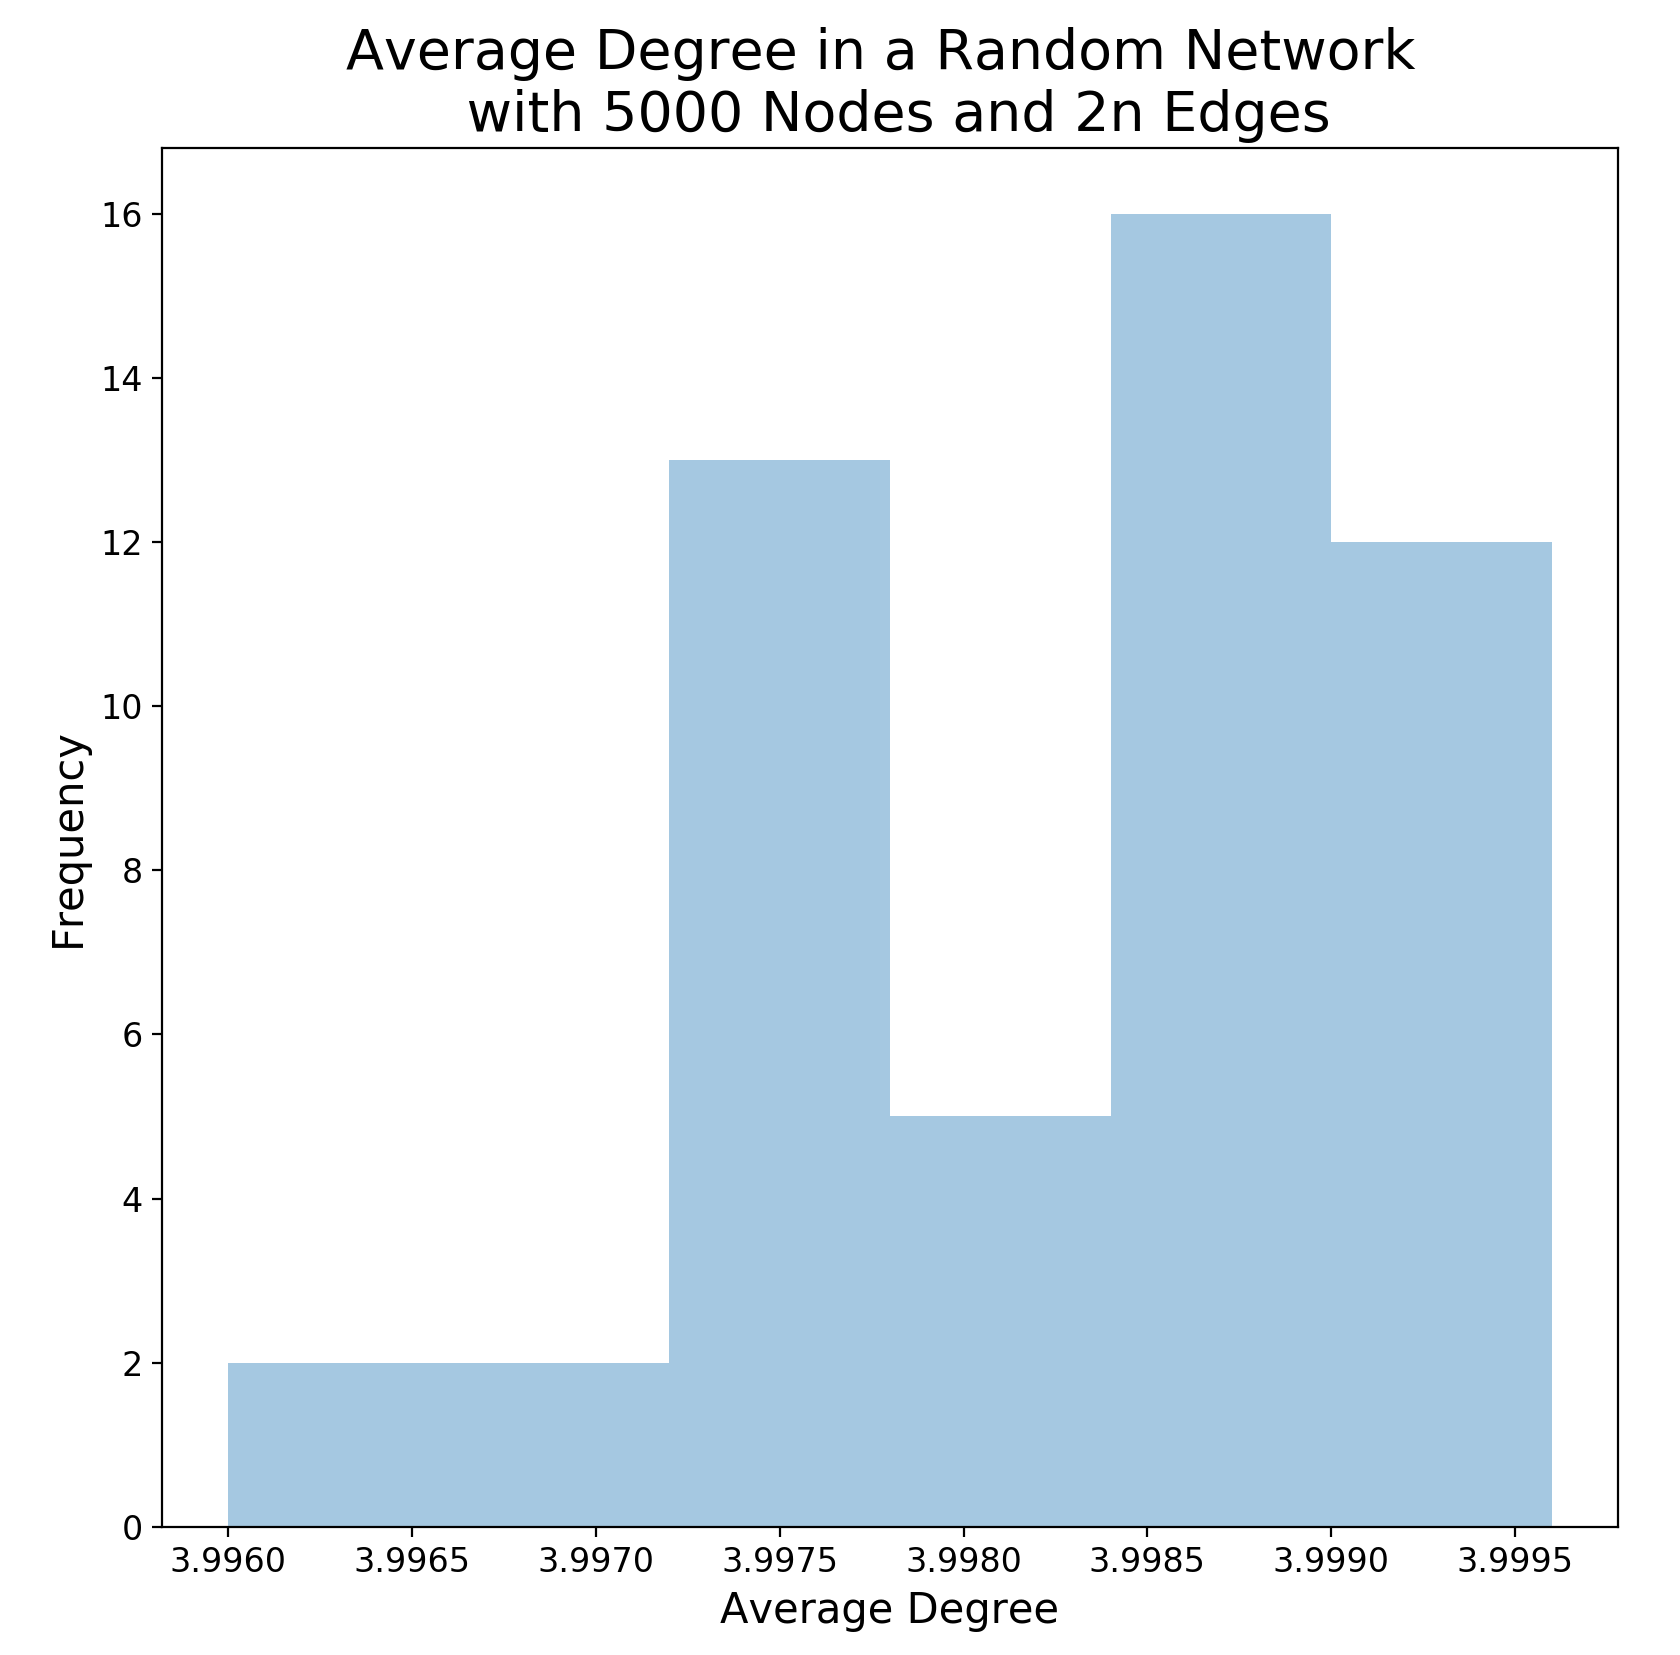
\includegraphics[width=\columnwidth]{images/r_deg_50.png}
    \captionof{figure}{Average degree in 50 runs where n=5,000, e=10,000}
    \label{fig:fifty_average_random_degree}
    \medskip
\endgroup

\bigskip
\bigskip
\bigskip

\begingroup
    \centering
    \medskip
    %width=\columnwidth
    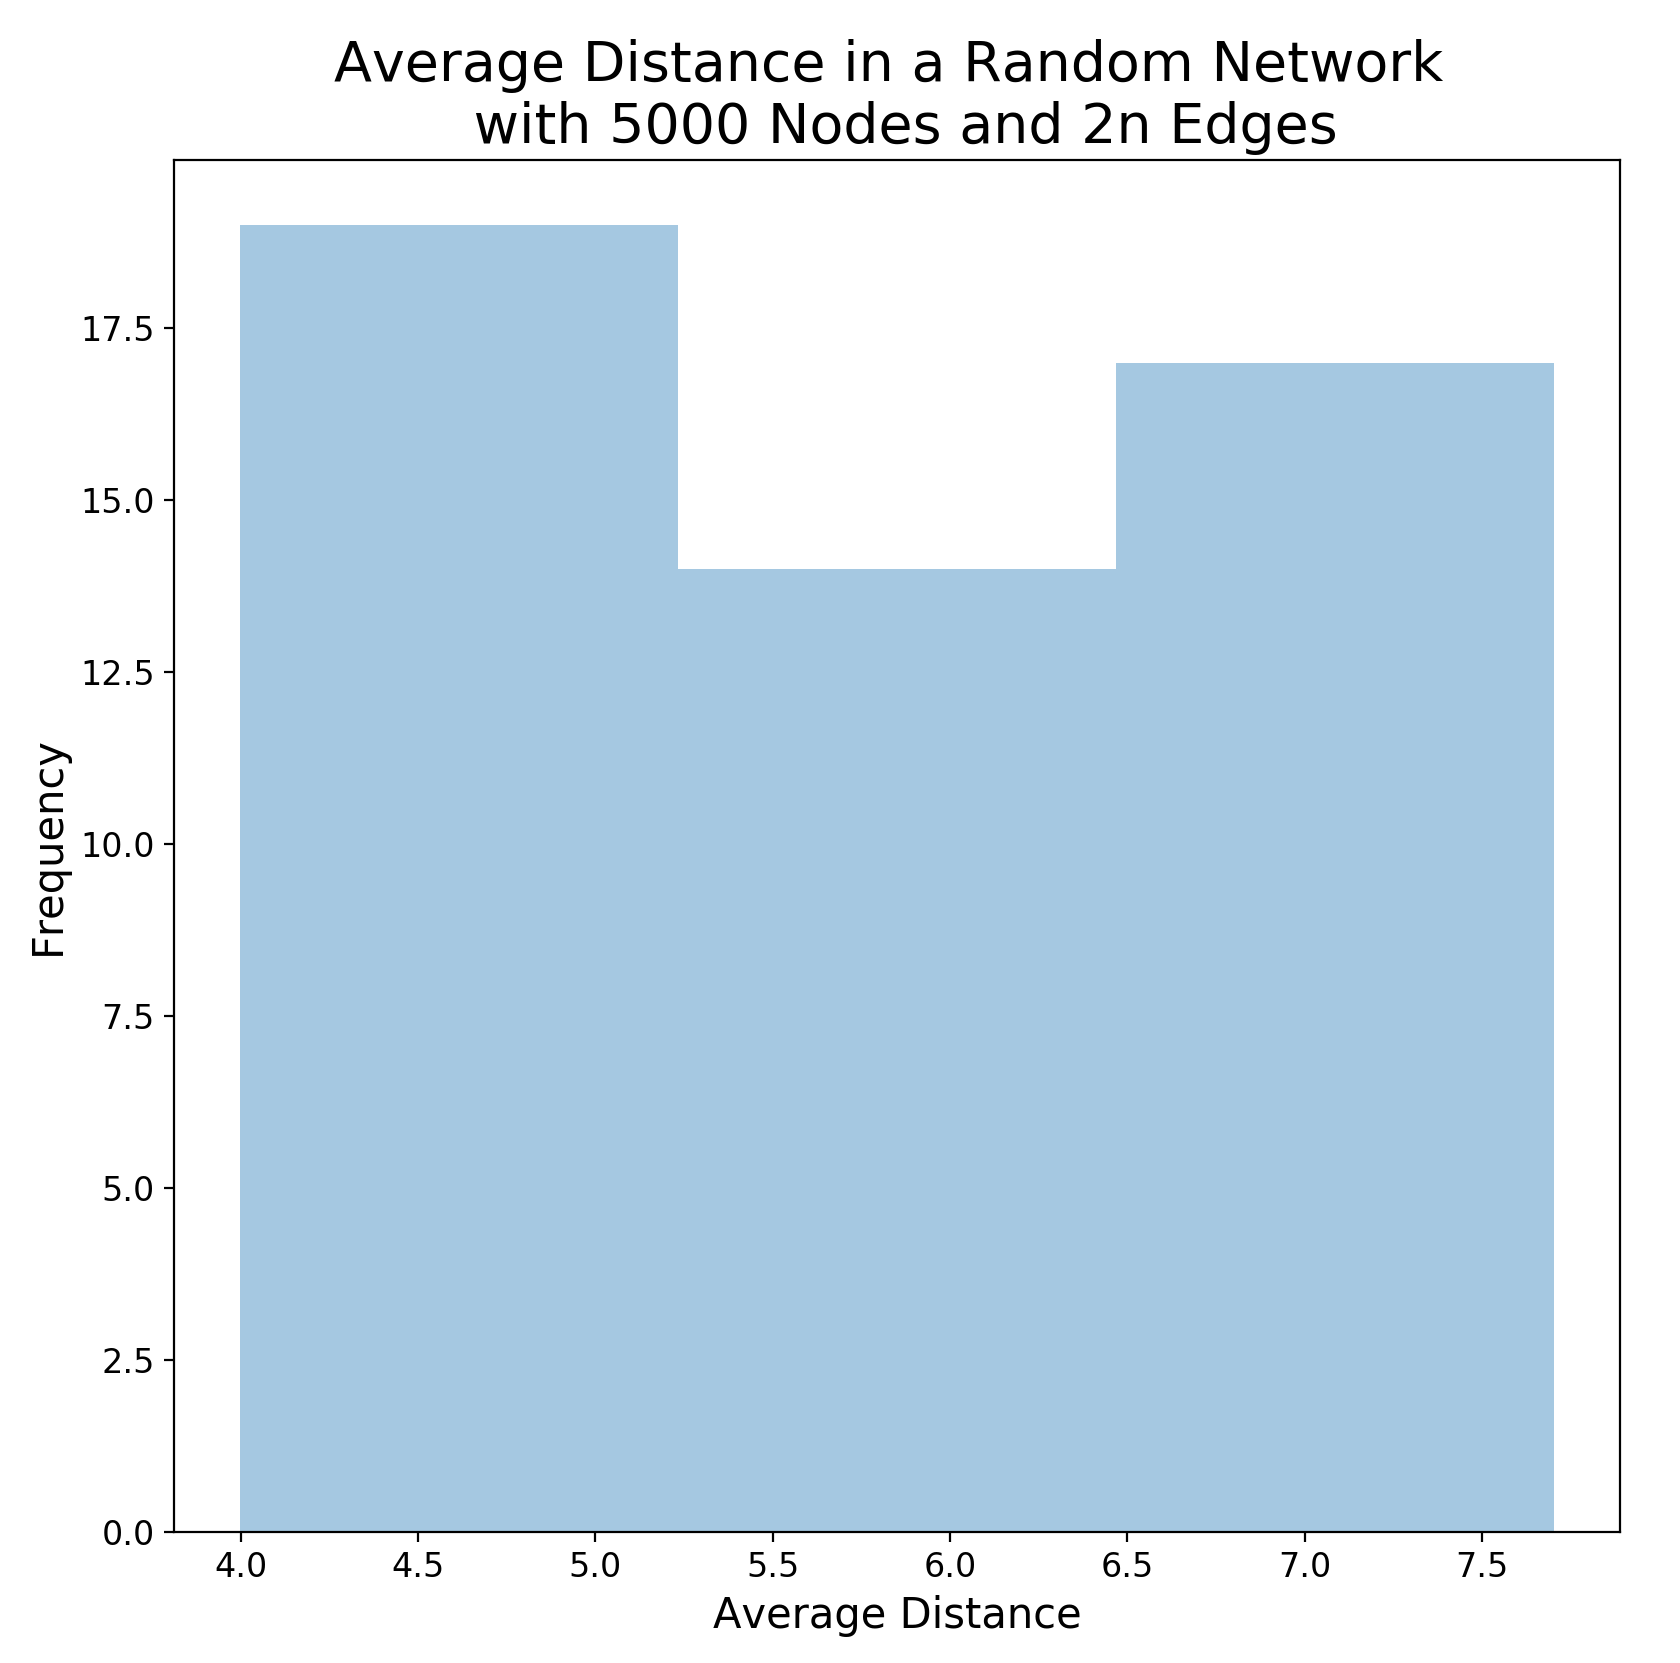
\includegraphics[width=\columnwidth]{images/r_dist_50.png}
    \captionof{figure}{Average distance in 50 runs where n=5,000, e=10,000}
    \label{fig:fifty_average_random_distance}
    \medskip
\endgroup

\newpage

\subsection{Scale-Free Network}

\noindent Figure \ref{fig:scalefree_histogram} depicts the results of five runs with 500 nodes and 1500 edges growing a scale-free network, while Figure \ref{fig:scalefree_network} shows a node visualization of a single run.

\begingroup
    \centering
    \medskip
    %width=\columnwidth
    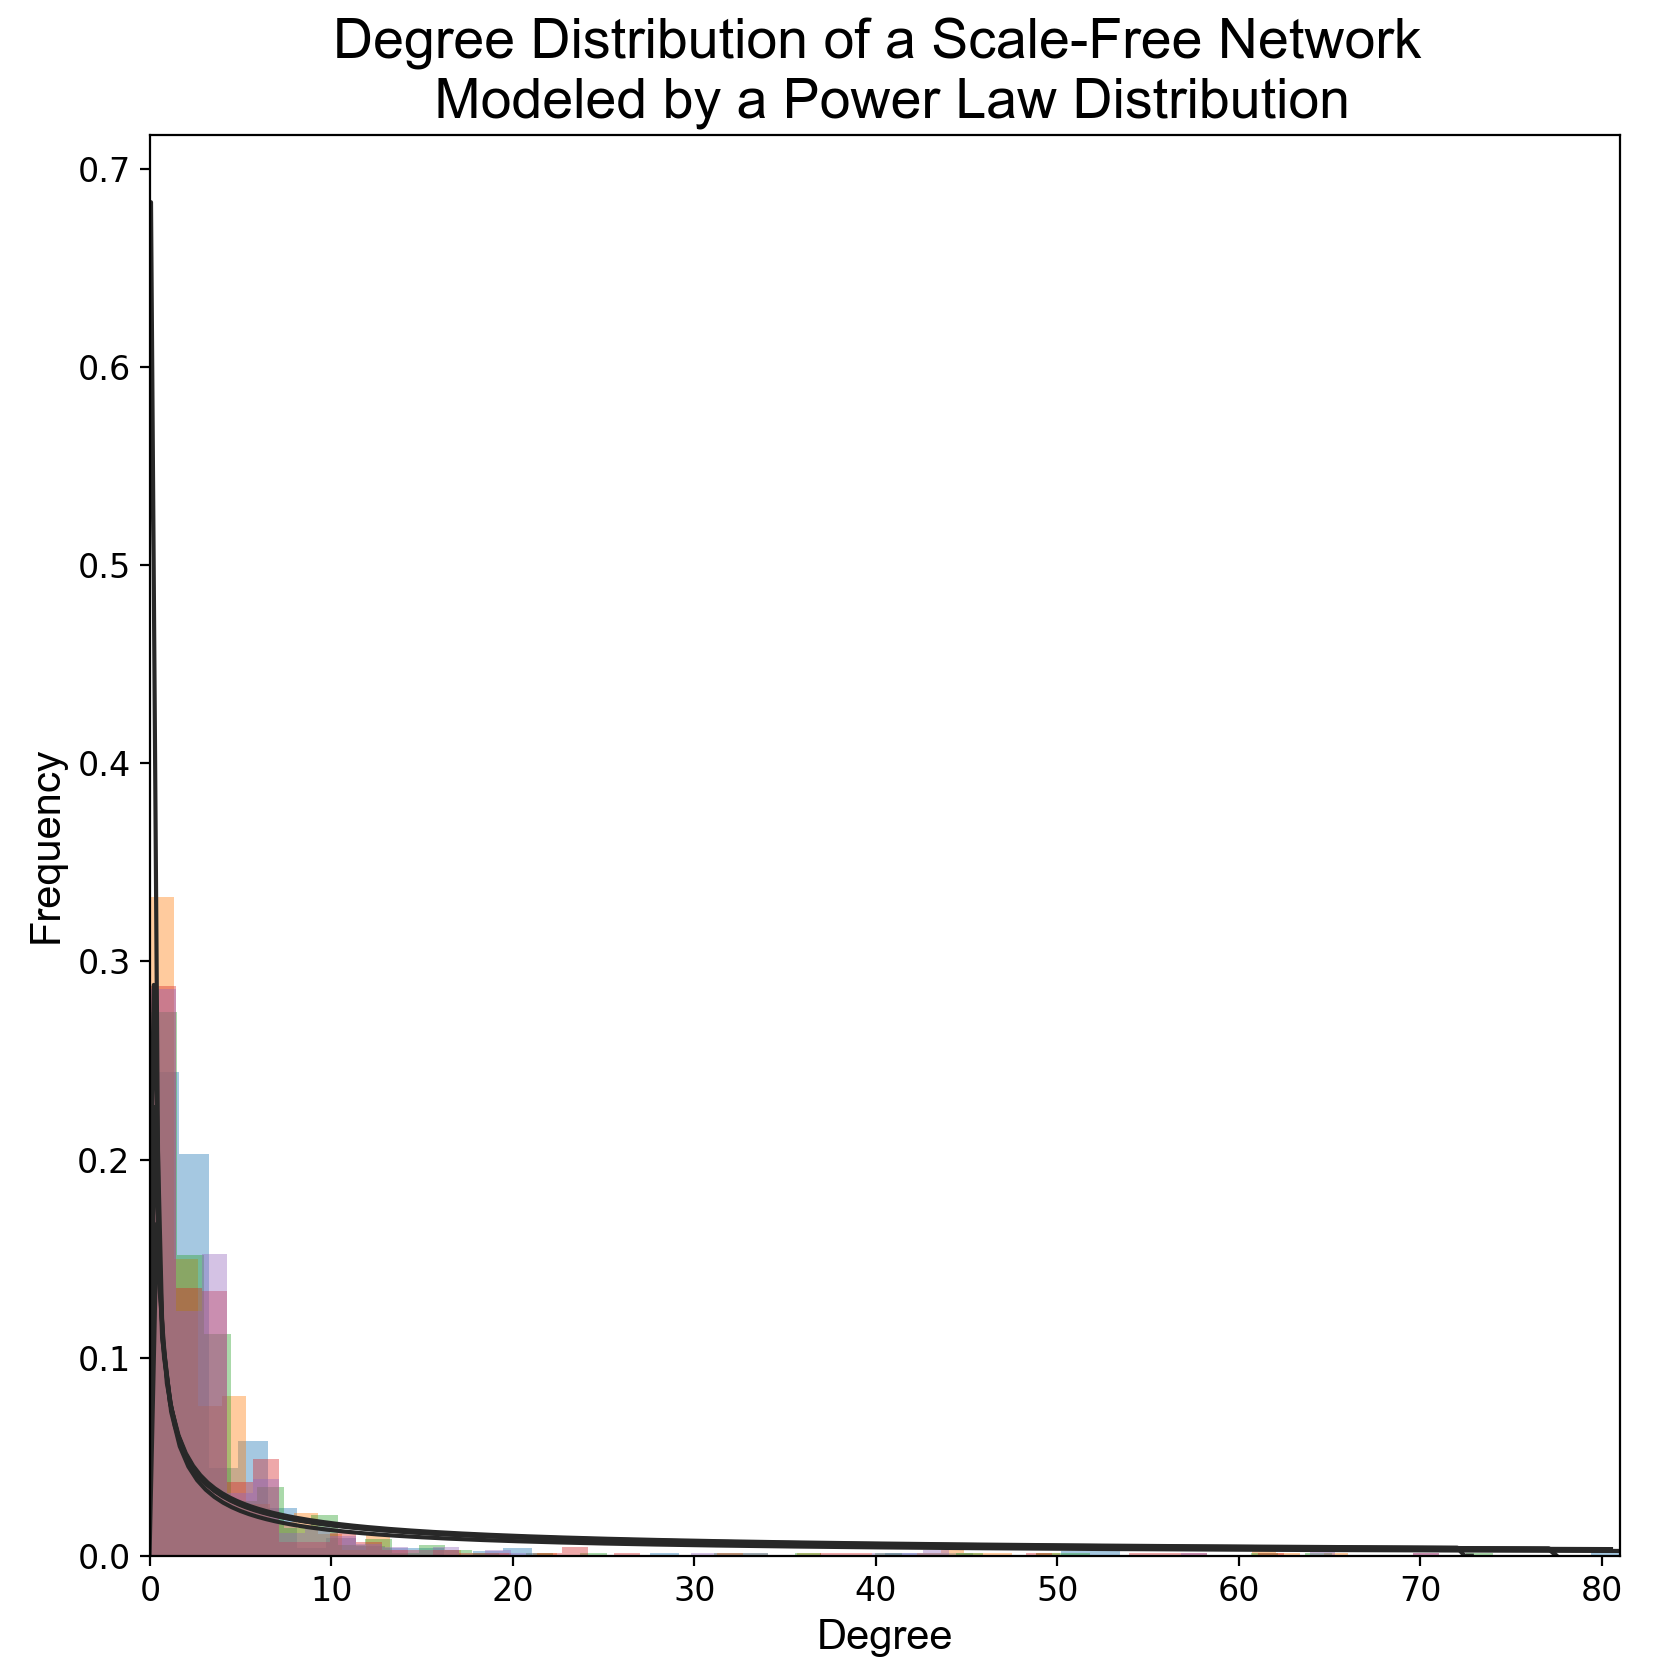
\includegraphics[width=\columnwidth]{images/sf_dist_5.png}
    \captionof{figure}{Five overlayed histograms of scale-free networks with n=500, e=1500}
    \label{fig:scalefree_histogram}
    \medskip
\endgroup

\bigskip
\bigskip
\bigskip

\begingroup
    \centering
    %width=\columnwidth
    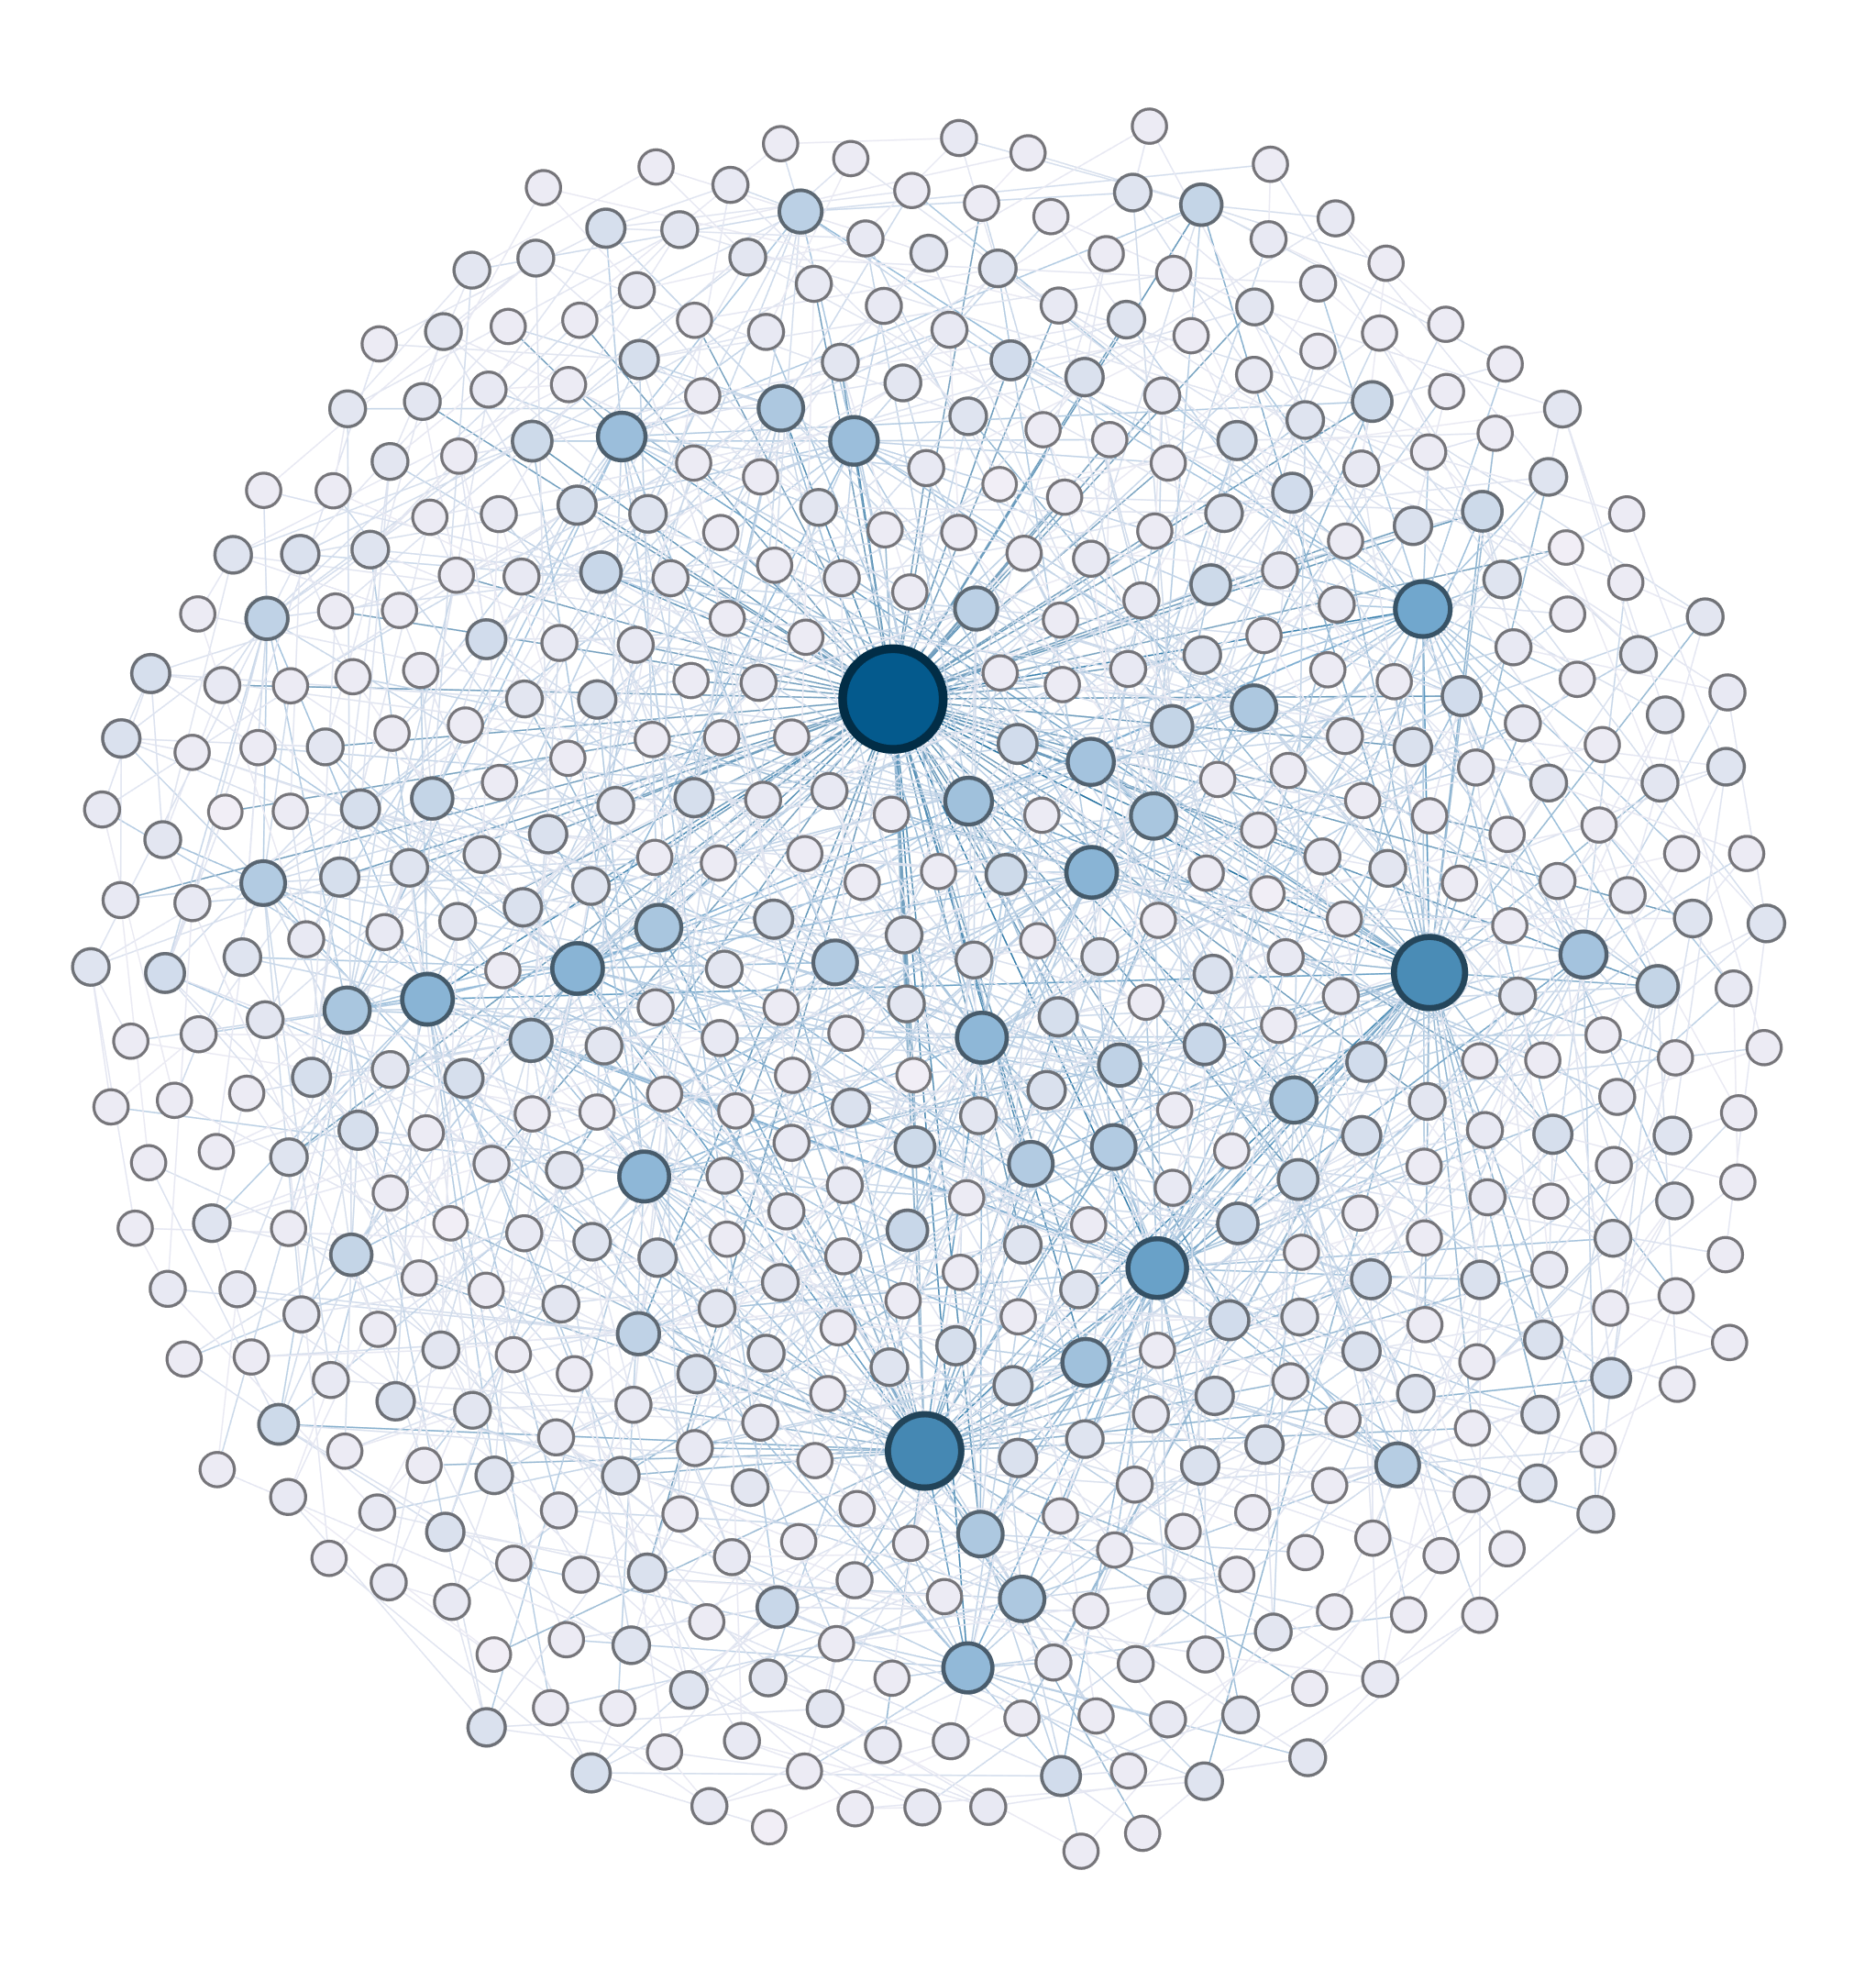
\includegraphics[width=\columnwidth]{images/scale-free.png}
    \captionof{figure}{Scale-free network with n=500, e=1500. Size and color of each is proportional to that node's degree. Bigger and darker node have more connections. Smaller and lighter nodes have fewer connections.}
    \label{fig:scalefree_network}
\endgroup

\newpage

\noindent Figure \ref{fig:fifty_average_scalefree_degree} shows the average degree in a scale-free network for 50 runs \ref{fig:fifty_average_scalefree_distance} shows the average distance in a scale-free network for 50 runs.

\begingroup
    \centering
    \medskip
    %width=\columnwidth
    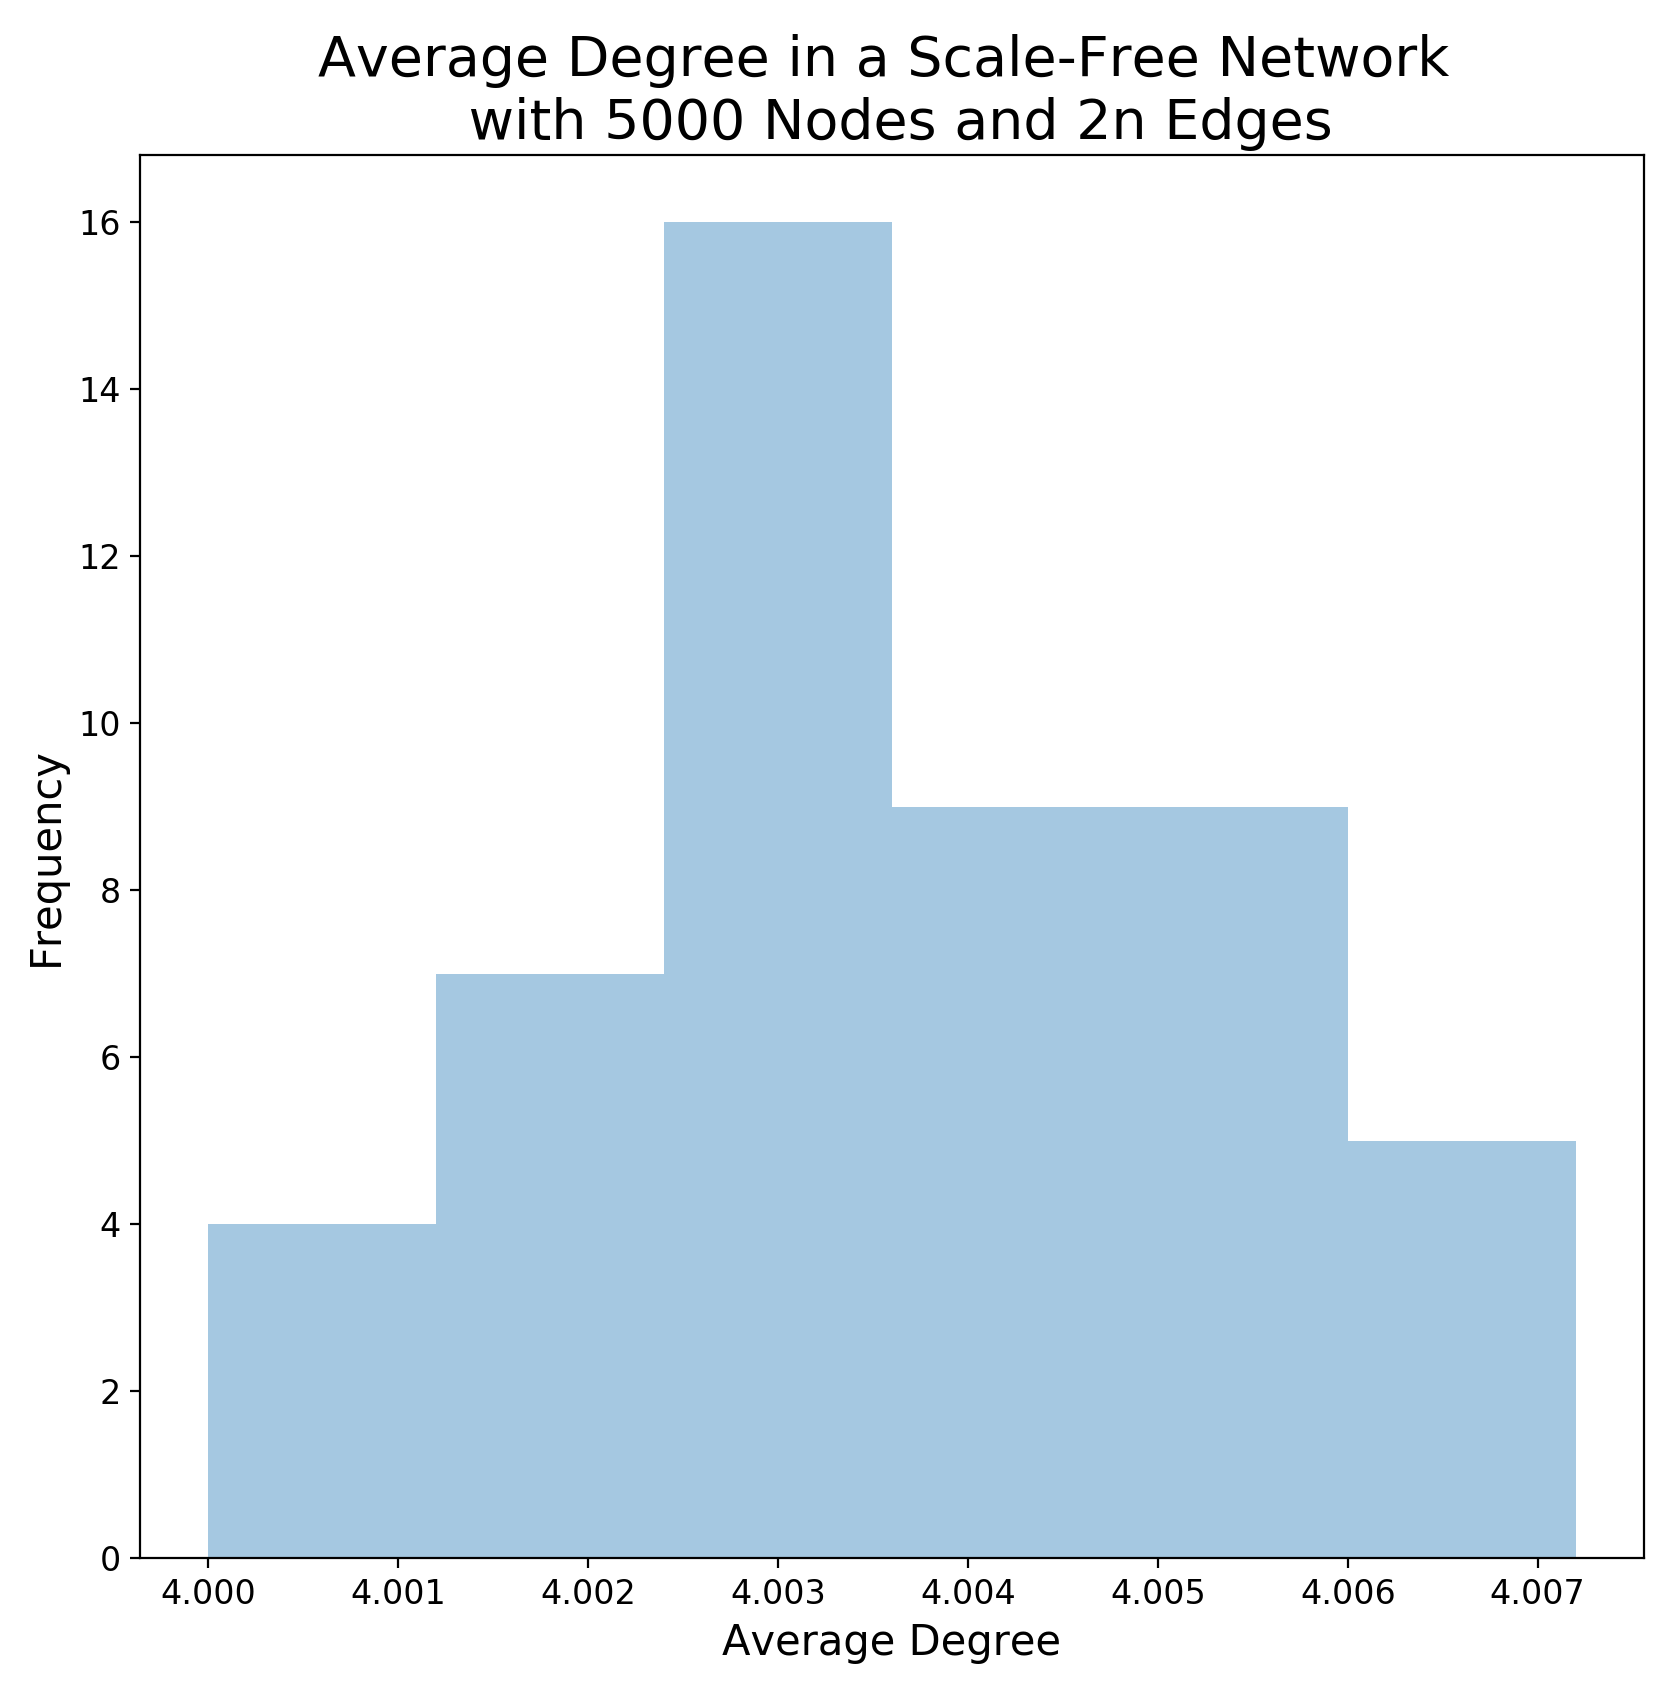
\includegraphics[width=\columnwidth]{images/sf_deg_50.png}
    \captionof{figure}{Histogram of average degree after 50 runs of a random network}
    \label{fig:fifty_average_scalefree_degree}
    \medskip
\endgroup

\bigskip
\bigskip
\bigskip

\begingroup
    \centering
    \medskip
    %width=\columnwidth
    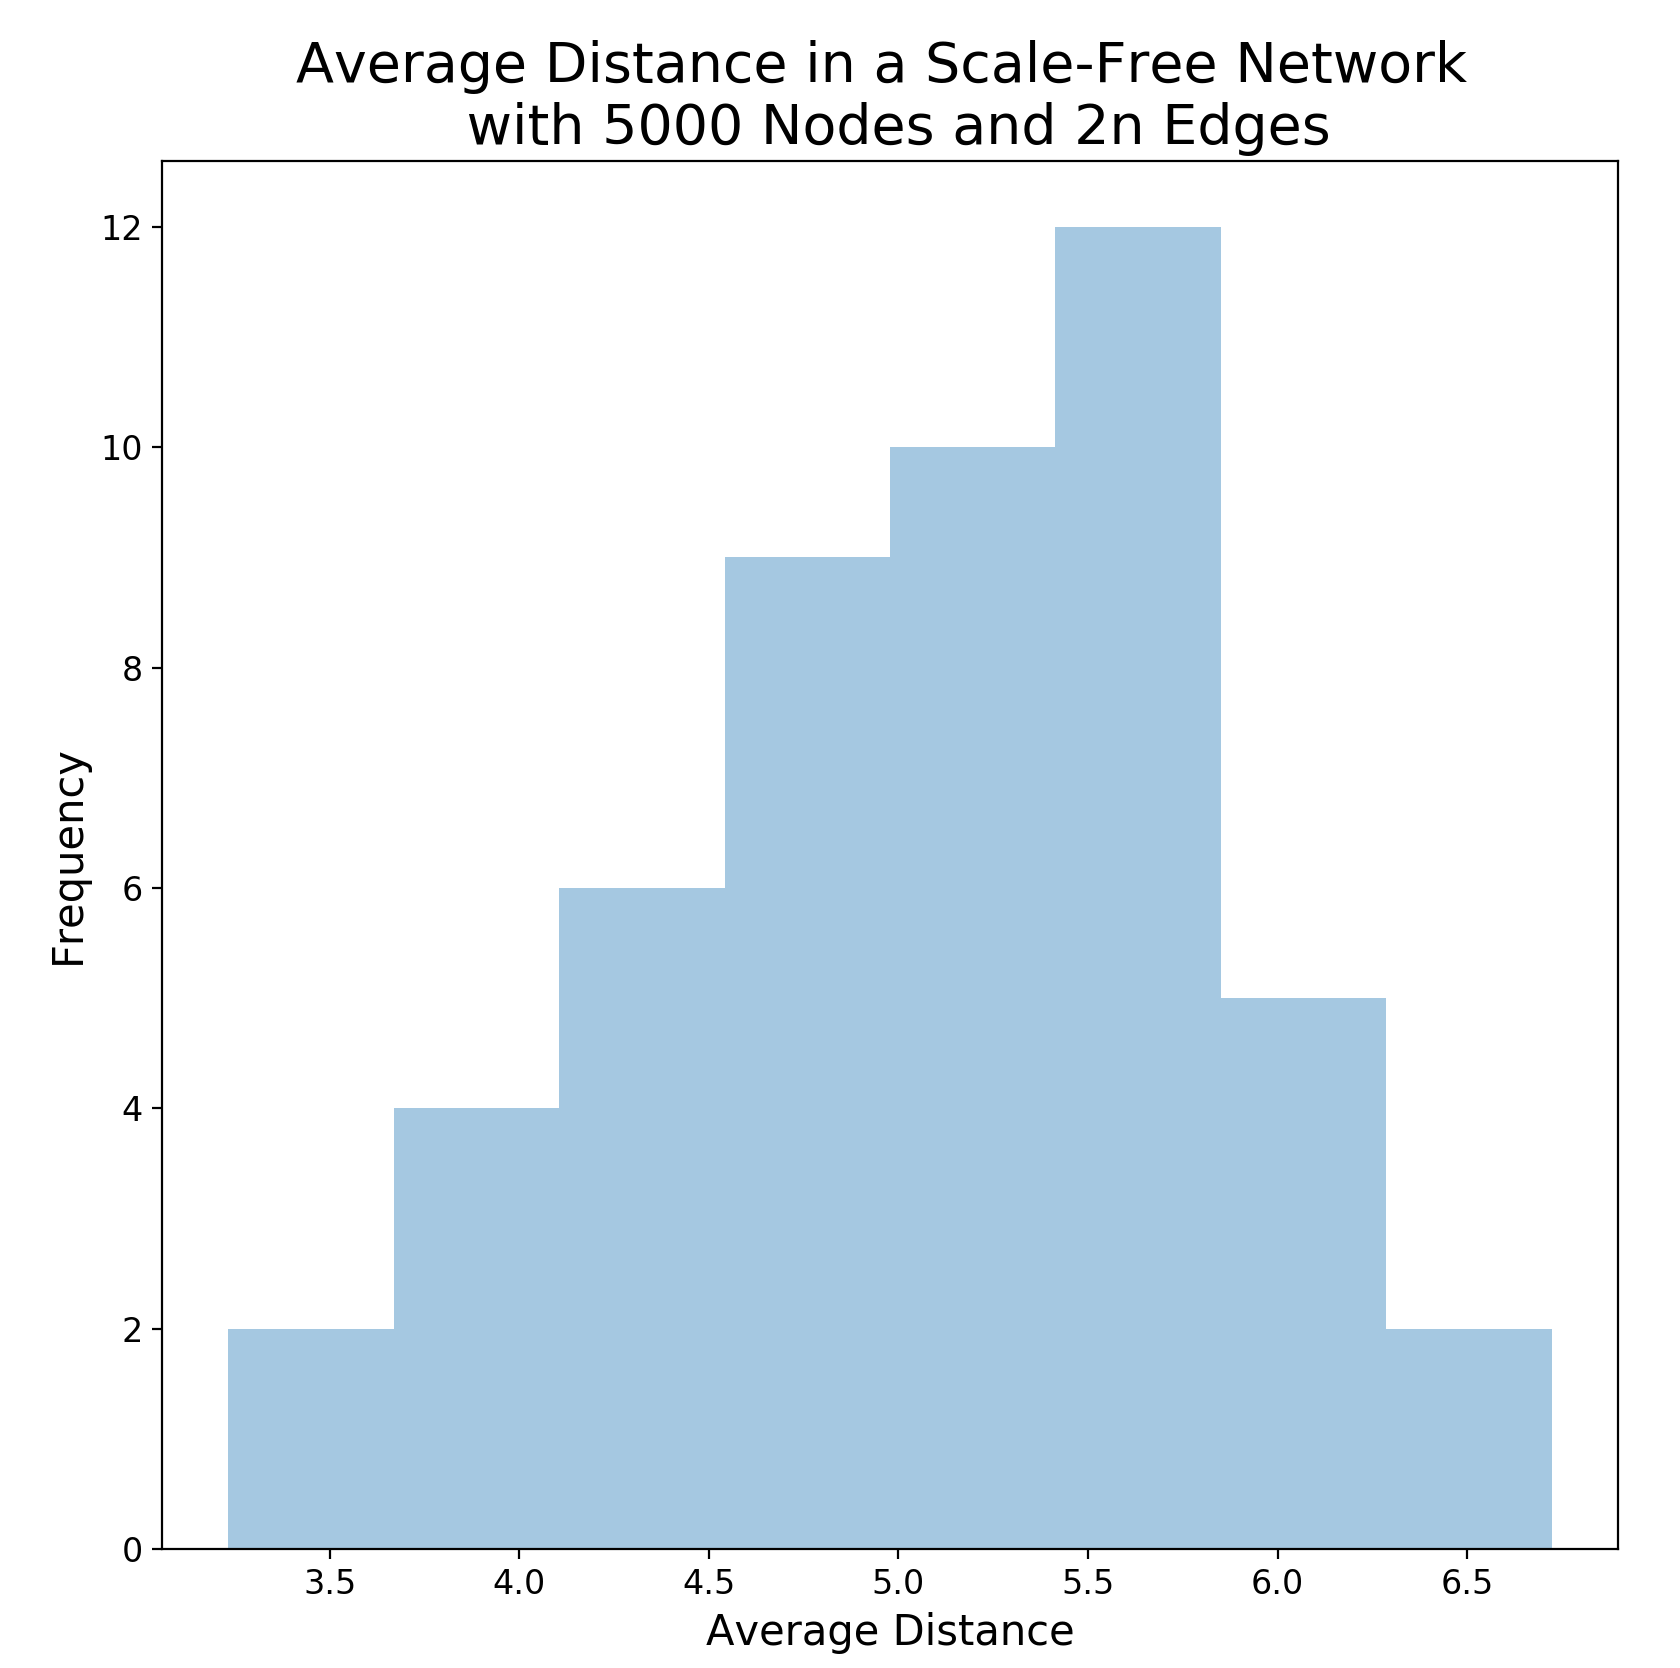
\includegraphics[width=\columnwidth]{images/sf_dist_50.png}
    \captionof{figure}{Histogram of average distance after 50 runs of a random network}
    \label{fig:fifty_average_scalefree_distance}
    \medskip
\endgroup


\newpage

\noindent Table \ref{table:random_table} shows the statistics of a single network of 5,000 nodes and 10,000 edges.
\medskip

\begingroup
    \medskip
    \centering
    \def\arraystretch{1.5}
        \begin{tabular}{lcc}
            \toprule
            & Random Network & Scale-Free Network \\
            \midrule
            Min. Degree    & 0      & 0         \\
            Max. Degree    & 16     & 226       \\
            Average Degree & 3.9988 & 3.0020    \\
            Variance       & 3.9848 & 56.0168   \\
            Fitting        & \lambda = 3.9988 & a = 0.1792, \gamma = 1.0000    \\ 
            \bottomrule
        \end{tabular}
    \captionof{table}{Statistics of a single network where \\ n = 5,000, e = 10,000}
    \label{table:random_table}
    \medskip
\endgroup

\bigskip

\noindent Table \ref{table:fifty_runs} shows the results of the 50 runs of 5,000 nodes and 10,000 edges.
\medskip

\begingroup
    \medskip
    \centering
    \def\arraystretch{1.5}
        \begin{tabular}{lcc}
            \toprule
            & Random Network & Scale-Free Network \\
            \midrule
            Avg. of Avg. Degree    & 3.9988    &  4.0035   \\
            Var. of Avg. Degree    & 7.6800$\times 10^{-7}$ & 3.1156$\times 10^{-6}$  \\
            Avg. of Avg. Distance  & 5.5694 & 5.0935    \\
            Var. of Avg. Distance  & 1.5507 & 0.5377   \\
            \bottomrule
        \end{tabular}
    \captionof{table}{Statistics of fifty runs where \\ n = 5,000, e = 10,000}
    \label{table:fifty_runs}
    \medskip
\endgroup

%%%%%%%%%%%%%%%%
%% Discussion %%
%%%%%%%%%%%%%%%%
\section{Discussion}

\noindent Empirically, the results obtained suggest that the random network follows a Poisson distribution, while the scale-free model follows a power law distribution. Despite the random and scale-free networks having a suspiciously similar average degree, the large variance in the scale-free model suggests a long tail. The large variance is a result of the random network having a maximum degree of 16, while the scale-free model has a maximum degree of 226. \\

\noindent While it was expected that the $\gamma$ parameter in the power law fit would lie between 2 and 3, the fitting resulted in $\gamma = 1 $, after adjusting for the mode of the dataset to be the minimum degree. 











\printbibliography

%%%%%%%%%%%%%%%%%%%%%%%%%%%%%%%%%%%%%%%%%%%%%
%%%%%%%%%%%%%%%%%%%%%%%%%%%%%%%%%%%%%%%%%%%%%
%%%%%%%%%%%%%%%%%%%%%%%%%%%%%%%%%%%%%%%%%%%%%

\newpage
\onecolumn
%%%%%%%%%%%%%%%%
%% Appendix %%
%%%%%%%%%%%%%%%%
\section{Appendix}

\subsection{Generating a Random Network}
\begin{lstlisting}[language=Python]
import numpy as np
import networkx as nx

def makeRandomNetwork(nodes, edges):

    if(edges > nodes*(nodes-1)/2):
        print("Too many edges")
        return None

    nodeArray = np.arange(nodes)
    edgeArray = np.zeros((edges, 2))

    for i in range(edges):
        n1 = np.random.randint(0,nodes)
        n2 = np.random.randint(0,nodes)
        while(n2 == n1):
            n2 = np.random.randint(0,nodes)
        edgeArray[i][0] = n1;
        edgeArray[i][1] = n2;

    G = nx.Graph()
    G.add_nodes_from(nodeArray)
    G.add_edges_from(edgeArray)

    return G
\end{lstlisting}


\subsection{Generating a Scale-Free Network - Version 2}
\begin{lstlisting}[language=Python]
import numpy as np
import networkx as nx

def makeScaleFreeNetwork(nodes, edges):

    if(edges > nodes*(nodes-1)/2):
        print("Too many edges")
        return None

    initialNodes = 10
    remainingNodes = np.arange(initialNodes, nodes)
    G = nx.complete_graph(initialNodes)

    for i in remainingNodes-initialNodes:
        n1 = i;
        n2Array = _selectNodes(G, int(edges/len(remainingNodes)) )
        for j in range(len(n2Array)):
            G.add_edge(n1, n2Array[j])

    return G

def _selectNodes(G, numConnections):

    networkNodeWeights = []
    selectedNodes = []

    for node in G.nodes():
        nodeDegree = G.degree(node)
        nodeProbability = nodeDegree / (2 * len(G.edges()))
        networkNodeWeights.append(nodeProbability)

    for i in range(numConnections):
        selectedNodes.append(np.random.choice(G.nodes(),p=networkNodeWeights))

    return selectedNodes
\end{lstlisting}


\subsection{Generating a Scale-Free Network - Version 1}
\begin{lstlisting}[language=Python]
import numpy as np
import networkx as nx

def generateNetwork(nodeSize, edgeBudget, name = "network"):

    # Check if given parameters make sense
    if(edgeBudget > nodeSize*(nodeSize-1)/2):
        print("Provided too many edges, please check the values")
        return None

    # Create an empty graph
    G = nx.Graph()
    G.name = name

    # For normalzing weights
    mappingRatio = float(1) / float(nodeSize)

    # Initialize all nodes to equal weights
    for m in range(nodeSize):
        G.add_node(m, weight = float(mappingRatio))

    # Edge budget loop counter
    i = 0

    while i < edgeBudget:
        weights = nx.get_node_attributes(G, 'weight')
        #print(weights)

        # For the first edge only
        if i == 0:
            # Choose any random two nodes
            n1 = np.random.randint(0, nodeSize)
            n2 = np.random.randint(0, nodeSize)

            # Choose another node if they are same
            while(n2 == n1):
                n2 = np.random.randint(0, nodeSize)

        else:
            # This returns an array but we want a single value, that is why
            #       we have [0] at the end
            n1 = np.random.choice(a = nodeSize, size = 1, replace = True, 
                p = list(weights.values()))[0]
            n2 = np.random.choice(a = nodeSize, size = 1, replace = True, 
                p = list(weights.values()))[0]

            # Choose another node if they are same
            while(n2 == n1):
                n2 = np.random.choice(a = nodeSize, size = 1, replace = True, 
                    p = list(weights.values()))[0]

        # This is for making sure that the edge was successfully added to the graph.
        #       Because networkx doesn't add if an edge already exists and it doesn't
        #       give any warning when there is a conflict
        oldEdgeCount = G.number_of_edges()
        G.add_edge(n1, n2, weight = 1)
        newEdgeCount = G.number_of_edges()

        if oldEdgeCount != newEdgeCount:
            #####################
            ## REWARD FUNCTION ##
            #####################
            # i+1 is used to prevent division by 0
            increaseRatio = float(mappingRatio) / float(10*(float(i+1))) 

            # Increase weights of the chosen nodes
            n_1_original_weight = float(weights[n1])
            n_2_original_weight = float(weights[n2])

            total_reduction = float(float(2) * increaseRatio)
            total_reduction_per_node = float(total_reduction / float(nodeSize - 2))

            for k in range(nodeSize):
                original_weight = float(weights[k])
                G.add_node(k, weight = 
                    float(float(original_weight) - float(total_reduction_per_node)))

            G.add_node(n1, weight = float(n_1_original_weight + increaseRatio))
            G.add_node(n2, weight = float(n_2_original_weight + increaseRatio))

            i = i + 1


    return G
\end{lstlisting}


\end{document}